\documentclass[a4paper,14pt]{article}
\usepackage{amsmath,amsfonts,amssymb,amsthm,epsfig,epstopdf,titling,url,array}
\usepackage[utf8x]{inputenc}
\usepackage[russian]{babel}
%\usepackage[T2A]{fontenc}
\usepackage{amsmath,amssymb,amsthm,amscd,amsfonts,graphicx}
\usepackage[14pt]{extsizes}

\usepackage{cleveref}
\usepackage{tikz}
\usetikzlibrary{arrows,shapes,snakes,automata,backgrounds,petri}

\newcommand{\workflow}{\textit{workflow}}
\newenvironment{definition}[1]{
\hskip \labelsep {\bfseries #1} \it}

\newtheorem{theorem}{Теорема}
\newtheorem{lemma}{Лемма}
\newtheorem{corollary}{Вывод}


\crefname{figure}{Рис.}{Рис.}
\crefname{lemma}{Лемма}{Леммы}
\crefname{theorem}{Теорема}{Теоремы}

\crefname{corollary}{Вывод}{Выводы}

\title{Дипломная работа}

\begin{document}
\maketitle
\textwidth 15.5cm
\topmargin -1cm
\parindent 1cm
\textheight 24cm
\parskip 1.5mm



\section{Введение}


Today’s scientific experiments typically in-
volve running and refining a series of intertwined computa-
tional analysis and visualization tasks on large amounts of
data. The complexity of these so-called analysis pipelines
resulting in high costs for development and maintenance,
the need for sharing knowledge encoded in these pipelines
as well as hardware to execute them, and the need for re
~\cref{fig:petri1}

За последних два десятилетия в научном сообществе компьютерное моделирование, названное eSience, стало незаменимой частью исследовательского процесса наравне с традиционными инструментами, такими как эмперические, основанное на  экспериментальных наблюдениях, теоретическое моделирование. Компьютерное моделирование включает в себя 

\subsection{Мотивация}
Мотивация
\section{Базовые понятия и определения}


\begin{definition}{Определение: Состояние}
Состояние любой системы или подсистемы в любой определённый момент времени характеризует, как система(продсистема) будет реагировать на входные данные.
Формально, под состоянием мы будем подразумевать всю накопленную системой информацию, которая влияет на поведение системы в текущий момент и в дальнейшие.
\end{definition}

\section{Формальное описание модели блок-ориентированных workflow}
В данном разделе будут введены базовые понятия, используемые в работе, в том числе
понятие атомарного блока,составного блока, графа связей, состояния workflow.

\subsection{Описанаие атомарного блока}
Базовой логической единицей потока данных является атомарный блок. Атомарный блок задаётся только недетерменированным конечным автоматом. 
 


Для примера рассмотрим простой блок типа Counter, который считает количество собственных запусков. У него разумеется есть состояние, и его реакция на входные данные из порта trigger зависит от того, сколько раз он уже сработал. Для подсчёта и хранения числа запусков он использует локальную переменную. И эту локальную переменную будем называть \textbf{переменной состояния}.
\\ 
В этом случае количество возможных состояний определяется типом счётчика. Если, к примеру, это int , то возможно только $2^{32}$ состояний, если double, то $2^{64}$. Если же тип счётчика  String, то число состояний бесконечно. Но не смотря на то что число состояний может быть очень болшим, логика переходов между ними достаточно проста. 

\subsubsection{Конечные автоматы}
Автоматом называется система , выходы которой зависят не только от поступивших входов, то и от текущего состояния системы.
% Состояние системы - объедие всей информации о предшествующих входах, необходимое системе для выполнения шага. 
Состояние системы может быть обозначено переменной состояния $s \in \Sigma$, где $\Sigma$  - это набор всех возможных состояний системы. Конечным автоматом называется автомат, для которого число состояний $\Sigma$ конечно.
\\
Внутренняя логика блока представляется моделью недетерминированного конечного автомата ( Finite State Machine, FSM)\\


Классическая теория конечных автоматов  (Hopcroft and Ullman, 1979) различает два вида автоматов: \textbf{Автомат Мили} и \textbf{Автомат Мура}. В Автомате Мили выходное значения сигнала явно зависит только от входных значений, в отличии от Автомата Мура, выходное значение сигнала в котором зависит лишь от текущего состояния данного автомата. Для полного задания автомата Мили или  Мура  дополнительно к законам функционирования, необходимо указать начальное состояние и оп­ределить внутренний, входной и выходной алфавиты. Между автоматами Мили и Мура существует соответствие, позволяющее преобразовать закон функционирования одного из них в другой или обратно. Автомат Мура можно рассматривать как частный случай автомата Мили, имея в виду, что последовательность состояний выходов автомата Мили опережает на один такт последовательность состояний выходов автомата Мура, т.е различие между автоматами Мили и Мура состоит в том, что в автоматах Мили состояние выхода возникает одновременно с вызывающим его состоянием входа, а в автоматах Мура - с задержкой на один такт, т.к в автоматах Мура входные сигналы изменяют только состояние автомата.\\
Определим недетерминированный автомат блока, который будет использоваться в работе.\\
\begin{definition}{Определение: Конечный автомат блока}Конечным автоматом блока называется набор $M = (\Sigma, I,\Lambda, T, s_{0})$ , где
\begin{enumerate}
\item[-] $\Sigma$ -набор конечных состояния,
\item[-] $I$ – набор доступных входных портов блока,
\item[-] $O$ - набор доступных выходных портов блока
\item[-] $s_{0} \in \Sigma$ - начальное состояние,
\item[-] $T: \Sigma \times 2^{I} \rightarrow  2^{\Sigma \times 2^{O}}$ отображение сопоставляющее каждому состоянию  и набору входных портов набор состояний с соответствующим набором выходных портов.
\end{enumerate}
\end{definition}


Как уже было определено выше, у блока имеется \textbf{начальное состояние} $s_{0}$, т.е. то в котором модель находится перед запуском. 
%Так же могут быть и \textbf{конечные сотояния}.
Визуально состояния соединены переходами, рядом с которыми указано, что проиходит при срабатывании работе.


\subsection{Графы связей workflow\\(Actor-Oriented Workflow Graphs)}

\begin{definition}{Граф связей workflow}
 Мультиграф связей workflow $W =(A, D)$ состоит из набора блоков $A$, представляющих задачи и набора связей , соединяющих блоки через порты. Блоки по своей сути явkяются пассивными, т.е. на набор входных данных выдают набор выходных данных на 
 Блоки передают друг другу токены данных через сообщающиеся порты.
\end{definition}

\begin{definition}{Порты}
Для каждого блока $a \in A$ существует собственный набор портов $port(a)$, таких что каждый порт $p \in ports(a)$ является либо входящим , либо выходящим для этого блока, т.е. $ports(a) = in(a) \cup out(a)$
%input/output signature ΣA of A, denoted A :: in(A) −→ out(A).3

\end{definition}

\begin{definition}{Связи}
Пусть для workflow $in(W) = {\bigcup_{a \in A} in(a)}$ будет набор всех входных портов, $out(W) = {\bigcup_{a \in A} out(a)}$ набором выходных портов соответственно. Тогда связь $d \in D$ будет направленным ребром $d = \langle o,i \rangle$
\end{definition}





\section{The Need for Composing Models of Computation in E-science}

\section{Workflows and Hierarchy}
Описание понятия  	акторa(actor,atomic actor.
,composite actor (a.k.a. sub-workflow))
\section{(Модели управления потоком)Models of Computation}
\subsection*{Process Networks (PN)}
\subsection{Использование PN}
\begin{enumerate}
\item[•] Тупики
\item[•] 
\end{enumerate}
Более подробно модель описывается  через Kahn networks.
Каждый актор запускается в отдельно треде(thread)(или вычислительном узле), и все акторы запускаются в конкурирующем режиме. 


\section*{SDF}
\subsection{Задачи}
\subsection{Использование SDF}
\begin{enumerate}
\item[] Deadlocks
\item[•] Consistency of data rates
\item[•] The value of the iterations parameter
\item[•] The granularity of execution
 Более подробно в секции 3.3.
\end{enumerate}
\subsection{Тупики(Deadlocks)}
\subsection{Consistency of data rates}
Все акторы внутри \textit{однородного(homogeneous)} SDF принимают только по одному токену из каждого входного порта и выписывают по 1 токену в наждый выходно порт. В кадом цикле должить быть "сдерживающий" актор,  так что dataflow-граф будет ациклическим , если убрать все "сдерживающие" акторы. Схему запуска можно определить статически, например, через топологическая сортировка графа.
%\subsubsection{Количество итераций}
\subsection{Свойства SDF}
\par SDF не связан с временными событяиями. Для всех акторов,входящих в SDF,  поглощение токенов из входных портов, выполнение вычисленых операций и отправление токенов в выходные порты явсляется атомарной операцией. Запуск композитного актора соответствует одной итерации содержащейся в нём модели по предварительно вычисленной схеме(schedule). При это схема выполнения рассчитывается так, чтобы , и при бесконечном числе итераций в модели не возникали тупики и накопление токенов. 
\subsubsection{Вычисление схем запуска}
Вложенные друг в друга SDF модели , можно уплощать(flasttern),
Запуск последовательный, преимущзественно на одном узле.

\section*{FSM}
Конечные автоматы (Finite State Machines) 
\section*{DDF}


В этой модели управления вместо того, чтобы выдавать каждому актору отдельный тред, система управления запускает отдельный актор, когда необходимые удовлетворены его зависимости на входе.  Dataflow делятся на два типа, dynamic dataflow (DDF) и synchronous dataflow (SDF). В случае DDF, система управления динамически определяет  какой актор необходимо запустить в следующим, и следовательно составляет схему запуска(firing schedule) динамически во время работу. В случае SDF, сиситема управления 
\begin{enumerate}
\item[•] Сети Петри
\item[•] Анализ Сетей Петри
\item[•] Граф Карпа и Миллера 
\item[•] Marked Graphs
\item[•] Однородные dataflow
\item[•] Обобщённые dataflow
\item[•] Модели Kaна (Khan) для параллельных вычислений
\end{enumerate}

9.0  Специальная лексика
 Dataflow - поток данных 


10.0 Используема литература

\section{СЕТИ}
\subsection{Сети Петри}
Сети Петри широко используются для моделирования и исcледования динамических дискретных систем. 
И прежде чем рассмотреть рассмотреть частные случаи использования Сетей Петри, приведём описание их каноничной формы, согласно определению Петерсона [Pet81].
\par Сеть Петри представляет собой двудольный ориентированный граф, состоящий из вершин двух типов — \textit{позиций} и \textit{переходов}, соединённых между собой дугами. Вершины одного типа не могут быть соединены непосредственно. В позициях могут размещаться метки (маркеры), способные перемещаться по сети.\\
\begin{definition}{Определение: Cеть Петри}
Простой сетью Петри наызвается набор $PN = (S,T,F)$ , где
\begin{enumerate}
\item $S = \lbrace s_{1},\ldots,s_{n} \rbrace$ - множество \textit{позиций}
\item $T = \lbrace t_{1},\ldots,t_{r} \rbrace$ - множество \textit{переходов} таких, что $S \bigcap T = \varnothing$.
\item $F \subseteq \mu S \times T \times \mu S$ - отношение \textit{инцидентности} такое, что 
\begin{enumerate}
\item[•] $\forall \langle  Q_{1}^{'}, t_{1}, Q_{1}^{''} \rangle , \langle Q_{2}^{'}, t_{1}, Q_{2}^{''}\rangle \in F : \langle Q_{1}^{'}, t_{1}, Q_{1}^{''} \rangle \neq \langle Q_{2}^{''}, t_{2}, Q_{2}^{'}\rangle \Rightarrow t_{1} \neq t_{2};$
\item[•] $\lbrace t | \langle  Q_{1}^{'}, t_{1}, Q_{1}^{''} \rangle \in F \rbrace = T$
\end{enumerate}
\end{enumerate} 

\end{definition}

Условия в пункте 3 говорят , что для каждого перехода $t \in T$ существует единственный элемент $\langle Q^{'}, t, Q^{''} \rangle$, задающий для него входное множество $Q^{'}$ и  выходное множество $Q^{''}$. Дадим определение входному и выходному множеству.

\begin{definition}{Определение: Входное и выходное множества мест и переходов}
\par Пусть задана сеть $N = (S,T,F)$.
\begin{enumerate}
\item Если для некоторого перехода t имеем $\langle Q^{'}, t, Q^{''} \rangle \in F$ , то будем обозначать \\$\bullet t = Q^{'} = \langle s |t \in s \bullet \rangle , t  \bullet = Q^{''} = \langle s | t \in \bullet s \rangle$
\item  И соответственно\\$\bullet s = \langle t|s \in t \bullet \rangle , s \bullet = \langle t | s \in \bullet t \rangle$
\end{enumerate}

Будем говорить, что $\bullet t$ - входные , а $t \bullet$ - выходные позиции для перехода t. Таким образом, соласно определению, справедливо:\\ $\forall t \in T : \langle \bullet t, t, t \bullet \rangle \in F $.\\ Позиция s называтся инцидентной переходу t , если $s \in \bullet t$ или $s \in t \bullet$.

\end{definition}

Сети Петри имеют удобную графическую форму представления в виде графа, в котором места изображаются кружками, а переходы прямоугольниками. Места и переходы, причем место s соединяется с переходом t если $s \in \bullet t$ и t соеднияется с s если $s \in t \bullet$. 

Само по себе понятие сети имеет статическую природу. Для задания динамических характеристик используется понятие маркировки сети $M \in \mu S$, т.е. функции $M : S \longrightarrow N_{0}$, сопоставляющей каждому месту целое число. Графически маркировка изображается в виде точек, называемых метками (tokens), и располагающихся в кружках, соответствующих местам сети. Отсутствие меток в некотором месте говорит о нулевой маркировке этого места.

\begin{definition}{Определение: Маркированная сеть Петри}
Маркированной сетью Петри называется набо $(PN, M_{0})$, где
\begin{enumerate}
\item PN =(S,T,F) - сеть;
\item $M_{0} \in  \mu S$ - начальная маркировка.
\end{enumerate}
\end{definition}


Сети Петри были разработаны и используются для моделирования параллельных и асинхронных систем. При моделировании в сетях Петри места символизируют какое-либо состояние системы, а переход символизируют какие-то действия, происходящие в системе. Система, находясь в каком-то состоянии, может порождать определенные действия, и наоборот, выполнение какого-то действия переводит систему из одного состояния в другое.

Текущее состояние системы определяет маркировка сети Петри, т.е. расположение меток (токенов) в местах сети, т.е. $M  \in S \rightarrow N$. Под маркировко, представленной в виде: $1s_{1} + 2s_{2} + 1s_{3} + 0s_{4}$, понимаем, что в позиции $s_{1}$ находится 1 метка, 2 метки в $s_{2}$, 1 метка в $s_{3}$ и ни одной метки в $s_{4}$. Так же представление этой маркировки можно сократить до $1s_{1} + 2s_{2} + 1s_{3}$. Дл ясравнения двух маркировок, мы определяем частичный порыядок. 
\begin{equation}
 	\nonumber
	\forall_{M_{1}, M_{2}} M_{1} \leq M_{2}, если \forall_{s \in S}: M_{1}(s) \leq M_{2}(s).
\end{equation}
Выполнение действия в системе, в сетях Петри определяется как срабатывание переходов. Срабатывание переходов порождает новую маркировку, т.е. порождает новое размещение меток (токенов) в сети. 

Работа мариковочной сети Петри управляется наличием или отсутствием маркировочных токенов. В сети Петри срабатывает  переход t, в процессе которого c каждого входа $s \in \bullet t$ снимается  метка и каждому выходу $s \in t \bullet$ прибавляется метка.

\begin{definition}{Определение: Правило срабатывания переходов}
Пусть $\Sigma = (S,T,F, M_{0})$ маркировочная сеть.
\begin{enumerate}
\item Переход $t \in T$ считается возбуждённым при маркировке $M \in \mu S$, если кажое положение $s \in \bullet t$ имеет хотя бы одна метка;
\item Переход t, возбуждённый при маркировке M,  может сработать, приведя к новой маркировке $M^{'}$,  которая  получается путём поглощения метки на каждом позиции $s \in \bullet t$ и появления новой метки на каждой позиции $s' \in t \bullet$.
\end{enumerate}
\end{definition}


Для сети Петри $(S,T,F)$ и её текущей маркировки $M_{1} \in \mu S$ опишем следующие обозначения: 
\begin{enumerate}
	\item[-] $M_{1} \xrightarrow{t} M_{2}$: преход t при 	маркировке $M_{1}$ возбуждён и при его срабатывание приводит к маркировке $M_{2}$
	\item[-] $M_{1} \xrightarrow{} M_{2}$: существует переход t, такой что $M_{1} \xrightarrow{t} M_{2}$
	\item[-]  $M_{1} \xrightarrow{\sigma} M_{n}$: последовательность переходов $\sigma = t_{1}t_{2}t_{3}...t_{n-1} \in T^{*}$ переводящая маркировку $M_{1}$ в $M_{n}$ через набор (возможно пустой) промежуточных маркировок $M_{2},...,M_{n-1}$, т.е.:
	 $M_{1} \xrightarrow{t_{1}} M_{2} \xrightarrow{t_{1}} ... \xrightarrow{t_{n-1}} M_{n}$ \\
Маркировка $M_{n}$ называется \textit{достижимой} из $M_{1}$ (и имеет обозначение $M_{1} \xrightarrow{*} M_{n}$) тогда и только тогда, когда существует последовательность такая переходов $\sigma$, что $M_{1} \xrightarrow{\sigma} M_{n}$. Отметим, что пустая последовательность переходов тоже допустима, $M_{1} \xrightarrow{*} M_{1}$.\\
Когда же мы имеем сеть Петри с начальной маркировкой $(S,T,F, M_{0})$, то маркировка $M^{'}$ будет допустимой, если $M_{0} \xrightarrow{*} M^{'}$.
\end{enumerate}

\begin{definition}{Определение: Живость(Live)}
Маркированная сеть Петри (PN, M) называется живой,
 если для любой достижимой маркировки  $M^{'}$  и любого перехода t существует маркировка $M^{''}$ достижимая из маркировки $M^{'}$ и задействующая переход t.
\end{definition}

\begin{definition}{Определение: Ограниченность(Bounded), безопасность(Safe)}
Маркированная сеть Петри (PN, M) называется ограниченной,
 если для каждого положения s существует такое натуральное число n, что для каждой достижимой маркировки меток в этом положении  меньше n. Сеть называется безопасной, если максимальное число меток не превышает 1.
\end{definition}
 
 
\begin{definition}{Определение: Правильность(Well-formed)}
Cеть Петри PN называется правильной, если существует такая начальная маркировка $M_{0}$, что сеть(PN, $M_{0}$) будет живой и ограниченной.
\end{definition} 

\begin{definition}{Определение: Путь}
Пусть дана сеть Петри PN. Путь C из вершины  $n_{1}$ в вершину $n_{k}$ представляет собой последовательность вершин $\langle n_{1},n_{2},...,n_{k} \rangle$ такую, что  $\langle n_{i},n_{i+1},n_{i+2}  \rangle \in F$ для $1 \leq i \leq k-2$. \\Путь C называется \textit{простым}, если для любых двух вершин $n_{i}, n_{j} \in C$ выполняется: $i \neq j \Rightarrow n_{i} \neq n_{j}$. \\Путь C называется \textit{безконфликтным}, елидля любой положения $n_{j}$ и любого перехода $n_{i}$ , $n_{i}, n_{j} \in C$, выполняется $j \neq i-1 \Rightarrow n_{j} \not\in \bullet n_{i}$.\\
Для удобства введём оператор $\alpha$ над путями. Тогда для пути $C = \langle n_{1},n_{2},...,n_{k} \rangle$  $\alpha (C) = \lbrace n_{1},n_{2},...,n_{k} \rbrace$
\end{definition} 
 
\begin{definition}{Определение: Сильная связность(Strongly Connected)}
Сеть Петри называется сильно звязной, если для любой пары вершин x и y существует путь из x в y.
\end{definition} 
 
\begin{definition}{Определение: Свободный выбор(Free-Choice)} 
Сеть Петри обладает свойством свободого выбора, если для любых двух переходов $t_{1}, t_{2} \in T$ выполняется $\bullet t_{1} \cap \bullet t_{2} \neq \varnothing \Rightarrow \bullet t_{1} = \bullet t_{2}$
\end{definition} 
\textbf{ПРИМЕРЫ}

\begin{definition}{Определение: WF-сеть(Workflow-net)}
  Пусть дана сеть Петри PN = (S,T,F).
  \begin{enumerate}
    \item[-] Если PN - WF-сеть c входной позицией i, тогда для любой позиции $s \in S: \bullet s \neq \lbrace или s = i$, т.е. i -единственная входная позиция.
    \item[-] Если PN - WF-сеть c выходной позицией o, тогда для любой позиции $s \in S:  s\bullet \neq \lbrace или s = o$, т.е. o -единственная выходная позиция.
     \item[-] Если PN - WF-сеть и мы добавляем в PN переход $t^{*}$, соединяющий выходную позицию o и входную позицию i (т.е. $\bullet t^{*} = {o}, t^{*} \bullet = {i}$), тогда получившаяся сеть будет обладать сильной связностью.
 \end{enumerate}
 
Для WF-сети начальную маркировку с единственной меткой только во входной позиции i будем обозначать $М_{i}$, а маркировку с единственной меткой только в выходной позиции o соответственно $М_{o}$.
\end{definition}
	
\begin{definition}{Определение: Корректность(Soundness)}
	WF-сеть PN = (S,T,F) корректна тогда и только тогда, когда:
	  \begin{enumerate}
	  \item[(i)] Для каждой маркировки M ,достижимой из i, маркировка o так же достижима из M.
	  \begin{equation}
	  	\nonumber
	  	\forall{M}  (i \xrightarrow{*} M) \Rightarrow (M \xrightarrow{*} o)
	  \end{equation}
	  \item[(ii)] Маркировка o - единственная достижимая из i маркировка, имеющая хотя бы одну метку в позиции o.
	  \begin{equation}
	  	\nonumber
	  	\forall_{M}  (i \xrightarrow{*} M \wedge M \geq o) \Rightarrow (M = o)
	  \end{equation} 
	  \item[(iii)] В (PN,i) нет неживых переходов.
	  \begin{equation}
	  	\nonumber
	  	\forall_{t \in T} \exists_{M, M^{'}}   i \xrightarrow{*} M  \xrightarrow{t}M'
	  \end{equation}	   
	  \end{enumerate}
\end{definition}


\begin{figure}[here]
\centering
\begin{tikzpicture}[node distance=2.cm,>=stealth',bend angle=45,auto]

  \tikzstyle{place}=[circle,thick,draw=black!75,minimum size=6mm]
  \tikzstyle{red place}=[place,draw=red!75,fill=red!20]
  \tikzstyle{transition}=[rectangle,thick,draw=black!75,minimum size=4mm]

\begin{scope}[xshift=5cm]

  \path  (0, 0)   node[place, tokens =1][label=below:i]   (i)  {}
  	   ++(1,0)
  	   +(0, 1.5)   node[transition]   (t1)  {t1} edge[pre](i)
  	   +(0, 0)   node[transition]   (t2)  {t2} edge[pre](i)
  	   +(0, -1.5)   node[transition]   (t3)  {t3} edge[pre](i)
	   ++(1, 0)       
       +(0, 1.5)   node[place][label=below:c1]  (c1) 	{}  edge[pre](t1)
       +(0, 0)     node[place][label=below:c2]  (c2) 	{}	edge[pre](t2)
       +(0,-1.5)   node[place][label=below:c3]  (c3) 	{}	edge[pre](t3)
	   ++(1, 0)       
        +(1, 1.5)   node[transition]   			 (t4)  	{t4} edge[pre](c1) edge[post, bend left](c1)
        +(0, 0)    	node[transition]   			 (t6)  	{t5} edge[pre](c2) edge[pre](c3)
       ++(1,0)
        +(0, 0)   node[place][label=below:o]  (o)	{}  edge[pre](t6) 
        ;
   \node[anchor=center] at (1.5, -4) {(a)};
\end{scope}

\begin{scope}[xshift=12cm]

  \path  (0, 0)   node[place, tokens =1][label=below:i]   (i')  {}
  	   ++(1,0)
  	   +(0, 0)   node[transition]   (t1')  {t1} edge[pre](i')
  	   ++(1, 0)          
       +(0, 1.5)   node[place][label=below:c1]  (c1') 	{}  edge[pre](t1')
       +(0, 0)     node[place][label=below:c2]  (c2') 	{}	edge[pre](t1')
       +(0,-1.5)   node[place][label=below:c3]  (c3') 	{}	edge[pre](t1')
	   ++(1, 0)       
       +(0, 1.5)   node[transition]   			(t2')  	{t2} edge[pre](c1')
       +(0, 0)    	node[transition]   			(t3')  	{t3} edge[pre](c2')
       +(0, -1.5)   node[transition]   	 	(t4')  	{t4} edge[pre](c3')
       ++(1, 0) 
       +(0, 0)     node[place][label=below:o]  (o') 	{}	edge[pre](t3')    edge[pre](t4')      
        ;
   \node[anchor=center] at (2.5, -4) {(b)};
\end{scope}

\end{tikzpicture}
\caption{This is a figure.}\label{fig:nonsound1}
\end{figure}


Рассмотрим примеры нарушения условий корректности WF-сетей.
\begin{enumerate}
  \item[-] Для WF-сети , изображённой на ~\cref{fig:nonsound1}(a) нарушено первое условие корректности. Срабатывание любого  из переходов t1,t2 или t3 приводит к маркировке, из которой маркировка o недостижима. При маркировке c1 мы имеем бесконечный цикл,а в случае маркировки c2 или с3 переход t5 никогда не сработает, т.к. требует по метке на каждой из входных позиций.
  \item[-] В результате выполнения последовательности переходов $\langle t1, t3,t4 \rangle$ WF-сети ~\cref{fig:nonsound1}(b) нарушается второе условие корректности, 
  \item[-] В сети , изображённой на ~\cref{fig:nonsound1}(b), так же нарушено третье условие корректности, т.к. переход t2 - неживой.
\end{enumerate}


Для данной WF-сети PN = (S,T,F) мы хоти определить, является ли она корректной. В [2] показано, как свойство корректности соотносится с живостью и ограниченностью сети. Для того, чтобы связать эти понятия,дадим определение расширеной сети $\overline{PN}= (\overline{S},\overline{T},\overline{F})$, где $
	\overline{S} =S, \overline{T} = T \cup \lbrace t^{*} \rbrace, \overline{F} = F \cup \langle o, t^{*} \rangle, \langle t^{*}, i \rangle \rbrace
$.


\begin{theorem}\label{thm:soundness}
WF-сеть PN кореектна тогда и только тогда, когда ($\overline{PN}$,i) - живая и ограниченная маркировочная сеть.
\end{theorem}

\subsection{Струтурные характеристики корректности}
Корректности WF-сети является её динамической характеристикой и из это вытекают некоторые проблемы:
\begin{enumerate}
	\item[-] Для сложных WF-сетей задача определения корректности может быть весьма затратной (Для произвольных WF-сетей вычисление ограниченности и живости имеет экспоненциальную сложность[8]).
	\item[-] ~\cref{thm:soundness} не определяет в какие именно компоненты WF-сети нарушают свойство корректности.
\end{enumerate} 
Поэтому полезно было бы знать какими структурными характеристиками обладают корректные WF-сети. Для этого будут рассмотрены некоторые классы WF-сетей: WF-сети со свободным выбором, хорошо структурированне WF-сети/
\subsubsection{WF-сети со свободным выбором}
Напомним определение свободного выбора в сети. Если для любых двух переходов $t_{1}, t_{2} \in T$, для которых выполняется $\bullet t_{1} \cap \bullet t_{2} \neq \varnothing$ , то необходимо чтобы $\bullet t_{1} = \bullet t_{2}$, т.е. эти переходы являются частью одного OR-split. \\
Соблюдение правила свободного выбора не мешает моделировать параллельное,последовательное и циклическое выполнение задач.\\
Если же мы будем допускать сети не обладающие свойством свободного выбора,то тогда на выбор между конкурирующими задчами влияет очерёдность в которой выполнялись предшествующие задачи, что является недопустимым при грамотном проектировании. 
 Нарушение свободы выбора,чаще всего возникает при сочетании распаралливания задач и маршрутизации с выбором.


\begin{figure}[here]
\centering
\begin{tikzpicture}[node distance=2.cm,>=stealth',bend angle=45,auto]

  \tikzstyle{place}=[circle,thick,draw=black!75,minimum size=6mm]
  \tikzstyle{red place}=[place,draw=red!75,fill=red!20]
  \tikzstyle{transition}=[rectangle,thick,draw=black!75,minimum size=4mm]

\begin{scope}[xshift=3cm]

  \path  (0, 0)   node[place, tokens =1][label=below:i]   (i')  {}
  	   ++(2,0)
  	   +(0, 0)   node[transition]   (t1')  {t1} edge[pre](i')
  	   ++(2, 0)          
       +(0, 1.5)   node[place][label=below:c1]  (c1') 	{}  edge[pre](t1')
       +(0,-1.5)   node[place][label=below:c2]  (c2') 	{}	edge[pre](t1')
	   ++(2, 0)       
       +(0, 1.5)   node[transition]   			(t2')  	{t2} edge[pre](c1')
       +(0, -1.5)   node[transition]   	 	(t3')  	{t3} edge[pre](c2')
       ++(2, 0) 
       +(0, 1.5)   node[place][label=below:c3]  (c3') 	{}  edge[pre](t2')
       +(0,-1.5)   node[place][label=below:c4]  (c4') 	{}	edge[pre](t3')
	   ++(2, 0)       
       +(0, 1.5)   node[transition]   			(t4')  	{t4} edge[pre](c3') edge[pre](c4')
       +(0, -1.5)   node[transition]   	 		(t5')  	{t5} edge[pre](c1') edge[pre](c4')  
       ++(2, 0)     node[place][label=below:o]  (o') 	{}	edge[pre](t4')    edge[pre](t5')      
        ;
\end{scope}

\end{tikzpicture}
\caption{This is a figure.}\label{fig:nonfreechoice1}
\end{figure}

На ~\cref{fig:nonfreechoice1} изображена такая ситуация. Сработавший переход t1 вводит параллелизм. Но тем не менее, в выбор между t2 и t5 ,т.к. переход t5 не возмуждён. Параллельное выполение t2 и t3 приводит к ситуации, когда выполнить переход t5 невозможно. Тем не менее, если выполение перехода t2 отложено до окончания выполнения t3, то тогда будет существовать выбор между t2 и t5. Но хотелось бы , чтобы параллелизм был отделён от выбора между альтернативами. Поэтому мы считаем конструкцию, приведённую на ~\cref{fig:nonfreechoice1}, неверной.



\begin{corollary}\label{crl:freechoicesoundness}
Для WF-сети со свободным выбором, задача проверки на корректность решается за полиномиальное время. 
\end{corollary}
\textit{Док-во.} Пусть PN - WF-сеть со свободным выбором, тогда $\overline{PN}$ тоже будет обладать  свобным выбором.  В работе [10] доказано, что определние живости и ограниченности для( $\overline{PN}$), можно за полиномиальное время. По ~\cref{thm:soundness} это эквивалентно корректности WF-сети.


\begin{lemma}
Корректная WF-сеть со свободным выбором - безопасная.
\end{lemma}
\textit{Док-во.} Пусть PN - корректная WF-сеть со свободным выбором. Тогда $\overline{PN}$ тоже будет со свобным выбором и правильностью(well-formed). Следовательно, $\overline{PN}$ S-покрываема[10], т.е. каждая позиция в . И т.к. в начальной маркировке есть всего одна метка,то ( $\overline{PN}$,i) будет безопасной,а следовательно и (PN,i).



Безопасность является предпочтительным свойством, т.к. нелогично было бы допускать несколько меток в позиции, представляющей состояние. Состояние может быть активным (1 метка) или неактивным (ни одной метки). 
 Non-
free-choice constructs such as the construct shown in Figure 4 are a potential source of
anomalous behavior (e.g., deadlock) which is difficult to trace.



\subsubsection{Хорошо структурированные WF-сети}
Другой подход для определения хорошей структурной характеристики workflow - это сбалансированность  компонент типов AND/OR-split и AND/OR-join. Очевидно, что два параллельных потока иницированных AND-split, не должны объединяться через OR-join.Так же как и два альтернативных потока ,  инициированных компонентом OR-split не должны синхронизироваться через AND-join.
\begin{figure}[here]
    \centering
    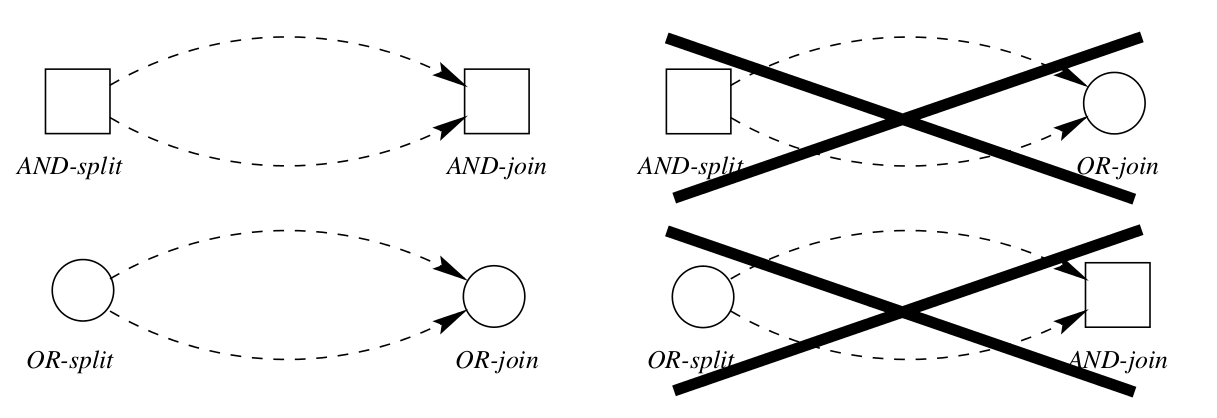
\includegraphics[width=\textwidth]{bad_joins.png}
    \caption{Хорошие и плохие конструкции}
    \label{img:bad_joins}
\end{figure}

Для того чтобы формализовать конструкции на рисунке ~\cref{img:bad_joins} дадим следующее определение.

\begin{definition}{Хорошая организованность(Well-handled)}
Сеть Петри PN  называется хорошо организованной, если для любых пар вершин x и y таких , что одна из вершин является позийцией , адругая переходом и для любой пары простых путей $C_{1}$ и $C_{2}$ из x в y, $\alpha (C_{1}  \cup \alpha (C_{2}) = \lbrace x, y \rbrace \Rightarrow C_{1} = C_{2}$.
\end{definition} 
Хорошая организованность может быть определена за полиномиальное время применяя алгоритмы vмаксимального потока и минимального среза , описанные в [5].

\begin{lemma}\label{lem:wellhandled}
Хорошая организованность сеть петри с сильной связностью будет хорошо организованной.
\end{lemma}
\textit{Доказательство.} Пусть PN - хорошая организованность сеть петри с сильной связностью. 
Очевидно, что не будет существовать ни одно пути 


\begin{definition}{Хорошая структурированность(Well-structured)}
WF-сеть является хорошая структурированной, если $\overline{PN}$ хорошая организованная.

\end{definition}




\begin{thebibliography}{10}
\bibitem{GG}[GG] Gray L., Griffeath D. The ergodic theory of traffic jams // J. Stat. 
\end{thebibliography}{10}

\end{document}
